% Copyright 2003 by Till Tantau <tantau@cs.tu-berlin.de>.
%
% This program can be redistributed and/or modified under the terms
% of the LaTeX Project Public License Distributed from CTAN
% archives in directory macros/latex/base/lppl.txt.


\section{Snakes}

\label{section-base-snakes}

\subsection{Overview}

A \emph{snake} is a ``way of adding a winding line to a path.'' To be
a bit more precise, you use snakes to extend the path and the
commands for using snakes start with |\pgfpath|. However, snakes do
not necessarily extend the path using line-to and curve-to operations;
rather, they can also contain move-to operations and, thereby, cause
the path to be split into many subpaths.

As an example, let us consider a simple snake like the |zigzag|
snake. It looks like this:

\begin{codeexample}[]
\begin{tikzpicture}
  \draw[snake=zigzag] (0,0)   -- (3,0);
  \draw[snake=zigzag] (0,-.5) -- (3,-1);
\end{tikzpicture}    
\end{codeexample}

The above example demonstrates the two key features of snakes:
\begin{enumerate}
\item
  Snakes are made up from little segments that are repeated several
  times. For the |zigzag| snake these segements look like this:
  \tikz{\draw[snake=zigzag] (0,0) -- (\pgfsnakesegmentlength+0.1pt,0pt);}.
\item
  Snakes ``follow along a straight to the target point.'' Thus, when
  the target point is not to the right of the start point, the snake
  is rotated appropriately.
\end{enumerate}


In order to use snakes, they first have to be \emph{declared}. This
declaration contains a detailed description of how each segement of
the snake looks like and in what ordering the different possible
segments are used.

Once a snake has been declared, it can be used. For this you specify a
target point and a snaked line will be added from the last point
current point to the target point.


\subsection{Declaring a Snake}


\subsubsection{Segments}

When you declare a snake, you provide a description of how the
different segments of the snake will be rendered. The description of
each segment should be given in a way as if the target of the snaked
line where at $(+\infty,0)$ and as if the segment's start where at the
origin. Thus, for example, the segment of the |zigzag| might be
defined using the following code: 
\begin{codeexample}[code only]
\pgfpathlineto{\pgfpoint{5pt}{5pt}}
\pgfpathlineto{\pgfpoint{15pt}{-5pt}}
\pgfpathlineto{\pgfpoint{20pt}{0pt}}
\end{codeexample}

\pgfname\ will ensure that an appropriate coordinate transformation
is in place when the snake segment is added to the path such that
the snake segment actually points in the right direction. Also
subsequent snake segments will be transformed such that they are
``further along the line'' toward the target. All transformations
are setup automatically.

Note that we did not use a |\pgfpathmoveto{\pgfpointorigin}| at the
beginning of the segment code. Doing so would subdivide the path into
numerous subpath. Rather, we assume that the previous segment caused
the current point to be at the origin.

While we can now describe segments, we still need a way to ``stop''
the snake. Also, \pgfname\ needs to know the width of the different
snake segments such that it can translate the next segment correctly.
Even though it would be possible to compute all this information
automatically, \pgfname\ does not do so and you have to provide the
information ``by hand'' for each segment. 


\subsubsection{Snake Automata}

Up to now our snakes only have one segment that is repeated again and
again. However, we might also like to have \emph{different} segments
and use rules to describe which segment should be used where. For
example, we might have special segments at the start and at the end.

For snakes we use a mechanism known in computer science as
\emph{finite automata} to describe which segment is used in each part
of the snake. The idea is the following: For the first segment we
start in a special \emph{state} called the \emph{initial state}. In
this state, and also in all other state later, \pgfname\ first
computes how much space is left on the snake. That is, \pgfname\ keeps
track of the distance to the target. Attached to each state there is a
set of rules of the following form: ``If the remaining distance is
less than $x$, switch to state~$q$.'' \pgfname\ checks for each of
these rules whether it applies and, if so, immediately switches to
state~$q$.

Only if none of the rules tell us to switch to another
state, \pgfname\ will execute the state's code. This code will add a
segment to the path. In addition to the rules there is also width
parameter attached to each state. \pgfname\ then translates the
coordinate system by this width and reduces the remaining distance.
Then, \pgfname\ either stays in the current state or switches to
another state, depending on yet another property attached of the
state.

The whole process stops when a special state called |final| is
reached. The segment of this state is added to the path immediately
(it is often empty, though) and the process ends.

\subsubsection{The Snake Declaration Command}

\begin{command}{\pgfdeclaresnake\marg{name}\marg{initial
      state}\marg{states}}
  This command declares a new snake called \meta{name}. The
  \meta{states} argument contains a description of the snake
  automaton's states and the transitions between them. The
  \meta{initial state} is the state in which the automaton starts.

  The \meta{states} argument should consist of |\state| commands, one
  for each state of the snake automaton. The |\state| command is
  defined only when the \meta{states} argument is executed.

\begin{codeexample}[]
\pgfdeclaresnake{example snake}{initial}
{
  \state{initial}[width=10pt]
  {
    \pgfpathlineto{\pgfpoint{0pt}{5pt}}
    \pgfpathlineto{\pgfpoint{5pt}{5pt}}
    \pgfpathlineto{\pgfpoint{5pt}{-5pt}}
    \pgfpathlineto{\pgfpoint{10pt}{-5pt}}
    \pgfpathlineto{\pgfpoint{10pt}{0pt}}
  }
  \state{final}
  {
    \pgfpathlineto{\pgfpoint{\pgfsnakeremainingdistance}{0pt}}
  }
}
\tikz{\draw[snake=example snake] (0,0) -- (3,0);
      \draw[snake=example snake] (0,-1) -- (3,-3);}
\end{codeexample}

  The |\state| command works as follows:
  \begin{command}{\state\marg{name}\oarg{options}\marg{code}}
    This command declares a new state inside the current snake
    automaton. The state is names \meta{name}.

    When \pgfname\ is in state \meta{name}, the following things
    happen:
    \begin{enumerate}
    \item
      The \meta{options} are parsed. This may lead, see below, to a 
      state switch. When this happens, the following steps are not
      executed. The \meta{options} are executed one after the other in
      the given order. If an option causes a state switch, the switch
      is immediate, even if later options might cause a different
      state switch.
    \item
      The \meta{code} is executed. When this happens, the coordinate
      transformation will be setup such that the origin is at the
      start of the segment and such that the target lies in the
      direction ``east.''
    \item
      After the \meta{code} has been executed, the state switches to
      whatever state has been specified inside the \meta{options}
      using the |next state| option. If no |next state| has been
      specified, the state stays the same.
    \end{enumerate}

    The following options are allowed inside the \meta{options}:
    \begin{itemize}
      \itemoption{switch if less than}|=|\meta{dimension}| to |\meta{new state}
      When this option is encountered, \pgfname\ checks whether the
      remaining distance to the target is less than
      \meta{dimension}. If so, an immediate state switch to \meta{new
        state} occurs.
      \itemoption{width}|=|\meta{dimension}
      This option tells \pgfname\ the width of the segment if it is
      appended to the path. The coordinate system will, afterward, be
      translated by \meta{dimension} to ensure that the next segment
      starts where the current one ended.

      In addition, this option will cause an immediate switch to the
      state |final| if the remaining distance is less than
      \meta{dimension}. The effect is the same as if you had said
      |switch if less than=|\meta{dimension}| to final| just before
      the |width| option.
      \itemoption{next state}=\meta{new state}
      After the segment has been added to the path, a state switch to
      \meta{new state} is performed. If this option is not given, the
      next state is the same as the current state.
    \end{itemize}

    There are two dimensions that are useful inside snake automata:
    \begin{command}{\pgfsnakeremainingdistance}
      This \TeX\ dimension holds the remaining distance to the target.
    \end{command}
    \begin{command}{\pgfsnakecompleteddistance}
      This \TeX\ dimension holds the distance already completed on the
      snake. 
    \end{command}
  \end{command}

  As a final example we present a more complicated snake that makes
  use of the different options:
\begin{codeexample}[]
\pgfdeclaresnake{complicated example snake}{initial}
{
  \state{initial}[width=5pt,next state=up]
  { \pgfpathlineto{\pgfpoint{5pt}{0pt}} }
  
  \state{up}[width=5pt,next state=down]
  {
    \ifdim\pgfsnakeremainingdistance>\pgfsnakecompleteddistance
      % Growing
      \pgfpathlineto{\pgfpoint{0pt}{\pgfsnakecompleteddistance}}
      \pgfpathlineto{\pgfpoint{5pt}{\pgfsnakecompleteddistance}}
      \pgfpathlineto{\pgfpoint{5pt}{0pt}}
    \else
      % Shrinking
      \pgfpathlineto{\pgfpoint{0pt}{\pgfsnakeremainingdistance}}
      \pgfpathlineto{\pgfpoint{5pt}{\pgfsnakeremainingdistance}}
      \pgfpathlineto{\pgfpoint{5pt}{0pt}}
    \fi%      
  }
  \state{down}[width=5pt,next state=up]
  {
    \ifdim\pgfsnakeremainingdistance>\pgfsnakecompleteddistance
      % Growing
      \pgfpathlineto{\pgfpoint{0pt}{-\pgfsnakecompleteddistance}}
      \pgfpathlineto{\pgfpoint{5pt}{-\pgfsnakecompleteddistance}}
      \pgfpathlineto{\pgfpoint{5pt}{0pt}}
    \else
      % Shrinking
      \pgfpathlineto{\pgfpoint{0pt}{-\pgfsnakeremainingdistance}}
      \pgfpathlineto{\pgfpoint{5pt}{-\pgfsnakeremainingdistance}}
      \pgfpathlineto{\pgfpoint{5pt}{0pt}}
    \fi%      
  }
  \state{final}
  {
    \pgfpathlineto{\pgfpoint{\pgfsnakeremainingdistance}{0pt}}
  }
}
\begin{tikzpicture}[snake=complicated example snake]
  \draw[snake] (0,0) -- (3,0);
  \fill[red!50,snake,rounded corners=2pt] (.5,-2) -- ++(2.5,-2.5)
                             [snake=none] -- ++(0,-.5) -| (0,-2) -- cycle;
\end{tikzpicture}
\end{codeexample}
\end{command}


\subsection{Using Snakes}

Two commands can be used to use a snake.

\begin{command}{\pgfpathsnakealongvector\marg{snake}\marg{length}\marg{vector}}
  This command will append the \meta{snake} to the current path. The
  length of the snake is given by \meta{length}. The \meta{vector}
  should be a normalizes vector (a vector having length |1pt|)
  pointing in the direction in which the snake should grow.
\begin{codeexample}[]
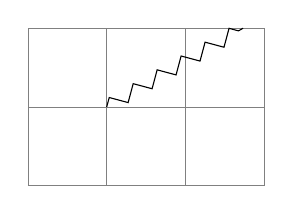
\begin{tikzpicture}
  \draw[help lines] (0,0) grid (3,2);
  \pgfpathmoveto{\pgfpoint{1cm}{1cm}}
  \pgfpathsnakealongvector{zigzag}{2cm}{\pgfpointpolar{30}{1pt}}
  \pgfusepath{stroke}
\end{tikzpicture}    
\end{codeexample}
\end{command}


\begin{command}{\pgfpathsnaketo\marg{snake}\marg{target}}
  This command will append the \meta{snake} to the current path such
  that it ends at \meta{point}. This command just calls the previous
  one after having computed the distance from the current point to
  \meta{target} and normalized the vector connecting the current point
  to the target.

  Note that the computation of the distance may be imprecise. In
  general, the placement precision of the snakes will not be perfect. 
\begin{codeexample}[]
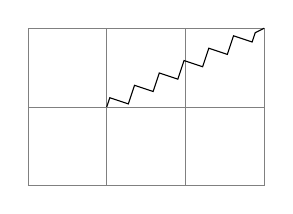
\begin{tikzpicture}
  \draw[help lines] (0,0) grid (3,2);
  \pgfpathmoveto{\pgfpoint{1cm}{1cm}}
  \pgfpathsnaketo{zigzag}{\pgfpoint{3cm}{2cm}}
  \pgfusepath{stroke}
\end{tikzpicture}    
\end{codeexample}
\end{command}

As was already mentioned, when each segment of the snake is added to
the path, an appropriate coordinate transformation will be in
force. It is sometimes useful to add an additional transformation
locally. For example, by reflecting everything around the $x$-axis
right before each segment is added, the snake will effectively be
mirrored along the path. The following command allows you to install
such a ``last minute transformation.''

\begin{command}{\pgfsetsnakesegmenttransformation\marg{code}}
  The \meta{code} will be executed at the very beginning of each
  segment. Normally, this be a transformation command that changes the
  $y$-axis in some way.
\end{command}




%%% Local Variables: 
%%% mode: latex
%%% TeX-master: "~/texmf/tex/generic/pgf/doc/pgf/version-for-pdftex/en/pgfmanual"
%%% End: 
